\documentclass[notitlepage]{svjour3}

\usepackage{graphics}
\usepackage{graphicx}
\usepackage[utf8]{inputenc}
\usepackage[T1]{fontenc}
\usepackage[american]{babel}
\usepackage{pgfplots}
\usepackage{amsmath}
\usepackage{tikz}
\usepackage{csquotes}
\usepackage{booktabs} % For formal tables.
\usepackage{authblk}
\usepackage{blkarray}
\usepackage{subcaption} % For subfigures.
\captionsetup{compatibility=false} % For subcaption.
\usepackage{tabularx}

\newtheorem{thm}{Theorem}[section]
\newtheorem{cor}[thm]{Corollary}
\newtheorem{lem}[thm]{Lemma}
\newtheorem{asp}{Assumption}%[section]
\newtheorem{defin}{Definition}[section]
\newtheorem{prop}{Proposition}[section]
\newtheorem{rem}{Remark}[section]
\newtheorem{alg}{Algorithm}[section]
\newtheorem{conj}{Conjecture}[section]
\newtheorem{comment}{Comment}[section]

\newcommand{\ind}[1]{1\hspace{-0.125cm}1\{#1\}}
\newcommand{\CR}{ {\mbox{\em CR}} }
\newcommand{\mv}{ {\mbox{v}} }

\newcommand{\SA}{ {\cal A} }
\newcommand{\SB}{ {\cal B} }
\newcommand{\SC}{ {\cal C} }
\newcommand{\SD}{ {\cal D} }
\newcommand{\SE}{ {\cal E} }
\newcommand{\SF}{ {\cal F} }
\newcommand{\SG}{ {\cal G} }
\newcommand{\SH}{ {\cal H} }
\newcommand{\SI}{ {\cal I} }
\newcommand{\SJ}{ {\cal J} }
\newcommand{\SK}{ {\cal K} }
\newcommand{\SL}{ {\cal L} }
\newcommand{\SM}{ {\cal M} }
\newcommand{\SN}{ {\cal N} }
\newcommand{\SO}{ {\cal O} }
\newcommand{\SP}{ {\cal P} }
\newcommand{\SQ}{ {\cal Q} }
\newcommand{\SR}{ {\cal R} }
\newcommand{\sS}{ {\cal S} }
\newcommand{\ST}{ {\cal T} }
\newcommand{\SU}{ {\cal U} }
\newcommand{\SV}{ {\cal V} }
\newcommand{\SW}{ {\cal W} }
\newcommand{\SX}{ {\cal X} }
\newcommand{\SY}{ {\cal Y} }
\newcommand{\SZ}{ {\cal Z} }
 
\newcommand{\bA}{ {\bf A} }
\newcommand{\bB}{ {\bf B} }
\newcommand{\bC}{ {\bf C} }
\newcommand{\bD}{ {\bf D} }
\newcommand{\bE}{ {\bf E} }
\newcommand{\bF}{ {\bf F} }
\newcommand{\bG}{ {\bf G} }
\newcommand{\bH}{ {\bf H} }
\newcommand{\bI}{ {\bf I} }
\newcommand{\bJ}{ {\bf J} }
\newcommand{\bK}{ {\bf K} }
\newcommand{\bL}{ {\bf L} }
\newcommand{\bM}{ {\bf M} }
\newcommand{\bN}{ {\bf N} }
\newcommand{\bO}{ {\bf O} }
\newcommand{\bP}{ {\bf P} }
\newcommand{\bQ}{ {\bf Q} }
\newcommand{\bR}{ {\bf R} }
\newcommand{\bS}{ {\bf S} }
\newcommand{\bT}{ {\bf T} }
\newcommand{\bU}{ {\bf U} }
\newcommand{\bV}{ {\bf V} }
\newcommand{\bW}{ {\bf W} }
\newcommand{\bX}{ {\bf X} }
\newcommand{\bY}{ {\bf Y} }
\newcommand{\bZ}{ {\bf Z} }
 
\newcommand{\mb}[1] { {\mbox{\rm #1}} }
\newcommand{\ee}{ {\mbox{e}} }
\newcommand{\diag}{ {\mbox{diag}} }
\newcommand{\bGamma}{ {\mbox{\boldmath $\Gamma$}} }
\newcommand{\bLambda}{ {\mbox{\boldmath $\Lambda}} }
\newcommand{\bOmega}{ {\mbox{\boldmath $\Omega$}} }
\newcommand{\bUpsilon}{ {\mbox{\boldmath $\Upsilon$}} }
\newcommand{\bPi}{ {\mbox{\boldmath $\Pi$}} }
\newcommand{\bPsi}{ {\mbox{\boldmath $\Psi$}} }
\newcommand{\bpi}{ {\mbox{\boldmath $\pi$}} }
\newcommand{\bphi}{ {\mbox{\boldmath $\phi$}} }
\newcommand{\bpsi}{ {\mbox{\boldmath $\psi$}} }
\newcommand{\balpha}{ {\mbox{\boldmath $\alpha$}} }
\newcommand{\bbeta}{ {\mbox{\boldmath $\beta$}} }
\newcommand{\bdelta}{ {\mbox{\boldmath $\delta$}} }
\newcommand{\bepsilon}{ {\mbox{\boldmath $\epsilon$}} }
\newcommand{\blambda}{ {\mbox{\boldmath $\lambda$}} }
\newcommand{\bgamma}{ {\mbox{\boldmath $\gamma$}} }
\newcommand{\bomega}{ {\mbox{\boldmath $\omega$}} }
\newcommand{\btau}{ {\mbox{\boldmath $\tau$}} }
\newcommand{\bnu}{ {\mbox{\boldmath $\nu$}} }
\newcommand{\bvarep}{ {\mbox{\boldmath $\varepsilon$}} }

\newcommand{\bxi}{ {\mbox{\boldmath $\xi$}} }
\newcommand{\bzeta}{ {\mbox{\boldmath $\zeta$}} }
\newcommand{\bvarphi}{ {\mbox{\boldmath $\varphi$}} }
\newcommand{\bkappa}{ {\mbox{\boldmath $\kappa$}} }
\newcommand{\bsigma}{ {\mbox{\boldmath $\sigma$}} }
\newcommand{\brho}{ {\mbox{\boldmath $\rho$}} }
\newcommand{\bvarrho}{ {\mbox{\boldmath $\varrho$}} }
\newcommand{\bPhi}{ {\bf \Phi} }

\newcommand{\boo}{ {\bf 0} }
\newcommand{\bzr}{ {\bf 0} }
\newcommand{\bon}{ {\bf 1} }
\newcommand{\ba}{ {\bf a} }
\newcommand{\bb}{ {\bf b} }
\newcommand{\bc}{ {\bf c} }
\newcommand{\bd}{ {\bf d} }
\newcommand{\be}{ {\bf e} }
\newcommand{\bff}{ {\bf f} }
\newcommand{\boldf}{ {\bf{f} } }
\newcommand{\bg}{ {\bf g} }
\newcommand{\bh}{ {\bf h} }
\newcommand{\bi}{ {\bf i} }
\newcommand{\bj}{ {\bf j} }
\newcommand{\bk}{ {\bf k} }
\newcommand{\bl}{ {\bf l} }
\newcommand{\bm}{ {\bf m} }
\newcommand{\bn}{ {\bf n} }
\newcommand{\bo}{ {\bf o} }
\newcommand{\bp}{ {\bf p} }
\newcommand{\bq}{ {\bf q} }
\newcommand{\br}{ {\bf r} }
\newcommand{\bs}{ {\bf s} }
\newcommand{\bt}{ {\bf t} }
\newcommand{\bu}{ {\bf u} }
\newcommand{\bv}{ {\bf v} }
\newcommand{\bx}{ {\bf x} }
\newcommand{\bw}{ {\bf w} }
\newcommand{\by}{ {\bf y} }
\newcommand{\bz}{ {\bf z} }

\providecommand{\keywords}[1]{\textbf{\textit{Keywords:}} #1}

\begin{document}

\title{P-score: a Reputation Bibliographic Index that Complements Citation Counts} 

\author{João Mateus de Freitas Veneroso \and Marlon Dias \and Alberto Ueda \and Sabir Ribas \and Berthier Ribeiro-Neto \and Nivio Ziviani \and Edmundo de Souza e Silva}

\institute{
 João Mateus de Freitas Veneroso \at
 Universidade Federal de Minas Gerais, Av. Pres. Antônio Carlos, 6627 - Pampulha, Belo Horizonte - MG, 31270-901,
 Departamento de Ciência da Computação, Sala 4304 \\
 Tel.: +55 (31) 99436-0909 \\
 \email{jmfveneroso@gmail.com} \and
 Marlon Dias              \at Universidade Federal de Minas Gerais \and
 Alberto Ueda             \at Universidade Federal de Minas Gerais \and
 Sabir Ribas              \at Universidade Federal de Minas Gerais \and
 Berthier Ribeiro-Neto    \at Universidade Federal de Minas Gerais \and
 Nivio Ziviani            \at Universidade Federal de Minas Gerais \and
 Edmundo de Souza e Silva \at Universidade Federal do Rio de Janeiro
}

\authorrunning{J. Veneroso, M. Dias, A. Ueda, S. Ribas, B. Ribeiro-Neto, N. Ziviani, and E. Silva} % if too long for running head

% \providecommand{\keywords}[1]{\textbf{\textit{Index terms---}} #1}

\maketitle

% \textbf{Declarations of interest: none} \\
\textbf{Conflict of Interest: The authors declare that they have no conflict of interest.} \\
% \\
% \\
% \textbf{Corresponding author:} \\
% João Mateus de Freitas Veneroso \\
% Mailing address: Universidade Federal de Minas Gerais, Av. Pres. Antônio Carlos, 6627 - Pampulha, Belo Horizonte - MG, 31270-901 \\
% Tel: +55 (31) 99436-0909 \\
% Email: jmfveneroso@gmail.com \\

\begin{abstract}
The notions of reputation and popularity in academia are critical for taking 
decisions on research grants, faculty position tenure, and research excellence awards. 
These notions are almost always associated with the publication track 
records of researchers. Thus, it is important to assess 
publication track records quantitatively. To quantify publication records, 
bibliographic indices are usually adopted and, among these, citation-based indices
such as the H-index are frequently considered. 
In this paper we study the correlation between P-score, a publication record index
and H-index, a very popular citation-based index, in the setting of conference 
ranking. While H-indices reflect the popularity of a given
publication or researcher in academia, P-scores can reflect the reputation of 
a publication or researcher among its peers, considering a reference set of 
reputable researchers. Popularity and reputation are frequently considered 
to be equivalent properties in the formulation of citation based indices, however 
these properties are not identical. Indeed, 
we first show that H-indices and P-scores are correlated with a Kendall-Tau coefficient 
that exceeds 0.5. However, we also notice that they show important differences. 
Particularly, we identify publication venues with high H-indices and low 
P-scores, as well as venues with low H-indices and high P-scores. We provide interpretations 
for these findings and discuss how they can be used by research funding councils and committees
to better support their funding decisions.
\end{abstract}

\keywords{P-score \and H-index \and Bibliographic Index \and Reputation Flows}

\section{Introduction}
\label{sec:introduction}

Academic research evaluation is a topic of interest to universities, research groups,
research funding institutions, and the public at large. An effective evaluation helps 
in the decisions regarding laboratory space allocation, research grants, tenure track, 
and university choice by students. It also 
has a direct impact on the reputation of universities and research institutions, which
affects their ability to attract the best possible talent. While evaluation of
academic research is complex, usually a function of multiple variables, a dominant variable in
most evaluation procedures is the research output of an institution. In particular, considerable
emphasis is given to the papers published by professors and students in this institution, as
well as the quality of these papers in terms of their impact on scientific knowledge. A
popular approach to the evaluation of scientific impact consists in comparing journals, 
conferences or papers with the usage of academic impact indices. Most often, these indices are based on 
the number of citations received by scientific publications, assuming that citation
counts act as a good proxy for research quality. However, this method has multiple shortcomings. 

First, in the evaluation and bibliometrics research communities, citations are understood
as a measure of popularity rather than a proxy for scientific impact, which is a similar but not
identical concept.
Second, citations can take a long time to happen. To illustrate this, in a recent
study that looked at first time to citation in a universe of more than a million papers, half the 
papers only received their first citation 20 months or more after they were
published~\cite{Nane2012}. Third, citations are not simple to compute and are not always broadly
available, particularly at the level of individual researchers.

Despite these limitations, citation-based indices continue to be a popular approach to
academic research evaluation~\cite{Kellner2008}.
Nonetheless, it is desirable to employ
complementary indicators that tackle the exposed problems without loss of effectiveness.

Academic reputation is an individual or group property strongly associated with 
academic impact, and while being similar it is not identical to academic popularity. An 
actor's popularity depends solely on the total number of endorsements
the actor receives from other actors, while its reputation or prestige depends on the 
reputations of the endorsing actors~\cite{Bollen2006}. Reputable venues tend to 
concentrate the most relevant research papers 
because that is how they acquire and keep their good reputations. At the same time, 
reputable authors seek to publish on reputable venues because it gives their 
research more visibility and accreditation. Therefore, researchers convey reputation
to a venue proportionally to their own reputation and the reputation of researchers
is proportional to the reputation of the venues where they publish.
This relationship between authors and venues constitutes a reputation network in which 
authors influence venue reputations and vice versa. 

{\em P-score}~\cite{Ribas2015a} is a graph-based modeling index that attributes quantitative
reputations to venues based on the publication patterns of a reference group of researchers,
without relying on citation information. Reputation is a subjective concept that can be 
quite difficult to define and quantify in the form of a bibliometric index. Thus,
instead of relying on a precise definition of reputation, P-score takes an agnostic 
view, exploiting the transference of this quantity called reputation among entities in order 
to identify the most reputable ones. The concept of reputation is determined by the choice of 
a reference group, which is presumed to be composed of reputable entities that act as sources
of reputation. P-score can deal with the three problems discussed previously. 

First, instead of measuring the amount of researcher attention, P-score measures reputations
which, under certain assumptions, provide a better proxy for academic impact as was shown by 
Ribas et al.~\cite{Ribas2015a}. Second, while citations can take years to happen, reputations 
tend to be established earlier on. As a consequence, the quality of new research can be 
promptly estimated using P-scores computed on the newest publication data. Third, P-scores do
not require citation data to be computed, which means that they can be recomputed quickly whenever 
one finds fit or convenient.

In this work, we show that the Pscores of conferences in Computer Science show a significant 
correlation with citation based indices, such as the H-index. Yet, there are important cases where 
the indices diverge. 
Our interpretation of these results are based on the intuition that while H-indices provide a 
quantification of the popularity of a publication or researcher among their peers, P-scores 
provide a quantification of the reputation of a publication or researcher among peers. When
P-scores and H-indices are strongly correlated, we have venues that are popular and of high
reputation or unpopular with a low reputation. Second, when P-scores are high (better rank position) 
and H-indices are low (worse rank position) we have venues of good reputation
that are associated with small research communities or subareas and are accordingly less popular. Third, when P-scores
are low (worse rank position) and H-indices are high (better rank position) we have venues of good popularity 
(usually associated with large research communities) that do not have
a high reputation (in the sense that the reference group of researchers does not publish frequently there).

\section{Related Work}\label{sec:related-work}

Quantitative measures of scientific impact have a long history. An influential approach is
Garfield's Impact Factor~\cite{Garfield1955a}, a journal-level measure that is defined
by the mean number of citations received by articles published in a given journal over a 2-year period. 
Despite being one of the earliest approaches at measuring scientific impact, it has showed remarkable 
survivability. 
Pinski et al. \cite{Pinski1976} describe several limitations with the Impact Factor. Impact factors also suffered 
criticism for being misleading~\cite{Nature2016,Saha2003} and for lacking reliable validation from an independent 
audit~\cite{Rossner2007}. Riikonen et al. \cite{Riikonen2008} showed that actual citation 
and publication counts were better predictors of a scientist's contribution than impact factors in a 
study that assessed the scientific contribution of Finnish researchers in biomedicine.

The acceptance rate is another important journal-level indicator that attempts to quantify scientific impact. It
is defined by the proportion of accepted papers relative to the number of submitted papers. Chen et al. \cite{Chen2010} 
have shown that highly selective conferences, the ones having low acceptance rates, have higher 
scientific impact measured in terms of the number of citations received by the published papers.

The H-index is an author-level index proposed by Hirsch~\cite{Hirsch2005}. Since its formulation, it has been 
widely adopted as a measure of individual scientific research output.
The H-index takes into account both the number of publications and the number of citations per publication, 
achieving higher values when a researcher obtains a consistently high number of citations over multiple publications. 
The H-index has been criticized for not taking into account field specific citation
statistics~\cite{Wendl2007}. The G-index, proposed by Egghe~\cite{Egghe2006}, is a less strict variation 
of the H-index.

Citation counts and derived measures are straightforward to calculate, but they represent only a coarse
estimate of academic impact, because they are essentially popularity measures. Some people are popular but not 
prestigious and vice versa. For example, an author of pulp detectives may sell many books, but may not have earned 
the respect of literary critics as pointed by Bollen et al.~\cite{Bollen2006}. Citations from 
prestigious journals are more relevant than citations from peripheral journals, as noted by Pinski et al.~\cite{Pinski1976}. To address this issue, some studies distinguish popularity from 
reputation or prestige with the usage of citation weighting strategies~\cite{Ding2011,Yan2011a} or 
Page Rank based methods~\cite{Bollen2006,Sun2007}. 
Furthermore, Piwowar~\cite{Piwowar2013} noted that citation-based indices are slow, since the 
first citation to a scientific article can take years to happen, concluding that the development of 
alternative indices to complement citation analysis is not only desirable, but a necessity.
As discussed by Leydesdorff~\cite{Leydesdorff2009}, each indicator has advantages and disadvantages 
deriving from their inherent biases.

Martins et al. \cite{Martins2009} proposed a method of assessing the quality of scientific conferences 
through a machine learning classifier that makes use of multiple features in addition to citations.
Gonçalves et al.~\cite{Goncalves2014} quantified the impact of various features on a 
scholar's popularity. They concluded that, even though most of the considered features are strongly correlated 
with popularity, only two features are needed to explain almost all the variation in popularity between different 
researchers: the number of publications and the average quality of the scholar’s publication venues. 

The idea of reputation, without the direct use of citation data, was discussed by Nelakuditi et al.~\cite{Nelakuditi2011}. 
They proposed a measure called \textit{peers' reputation} for 
research conferences and journals, which ties the selectivity of the publication venue based upon 
the reputation of its authors' institutions. The proposed measure was shown to be a better indicator 
of the selectivity of a research venue than the acceptance ratio.

\section{P-score: a Network Based Index} 
\label{pscore} 

Contrary to citation counts such as the Impact 
Factor~\cite{Garfield1955a,Saha2003,Thomson2017,Balaban2012} and 
H-index~\cite{Benevenuto2016,Bar-Ilan2008,Egghe2008,Bornmann2005,Bornmann2011}, 
P-scores are a graph-based modeling index that takes into account 
the relations among researchers, papers they published and their publication venues. They are based on a framework of \textit{reputation flows}~\cite{Ribas2015} which we describe in this section.

Let a \emph{reputation graph} be a graph with three node types of academic entities: (a) {\em reputation sources} representing groups of selected researchers, 
(b) {\em reputation targets} representing venues of interest, and
(c) {\em reputation collaterals} representing entities we want to compare such as research groups and academic 
departments. 
Figure~\ref{fig:overview} provides a generic illustration of our reputation graph and introduces the following 
notation: $S$ is the set of reputation sources, $T$ is the set of reputation targets, and $C$ is the set of reputation collaterals.

\begin{figure}[ht]
   \centerline{
\includegraphics[scale=0.6]{figures/overview-line}}
   %\centerline{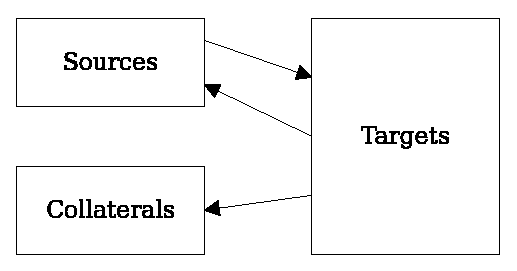
\includegraphics[scale=0.6]{figures/models/overview}}
   \caption{Structure of the reputation graph.}
   \label{fig:overview}
\end{figure}

The reputation of source nodes influences the reputation
of target nodes as much as the reputation of target nodes
influences the reputation of source nodes. Note that the
reputation of target nodes also influences the reputation of
collaterals, but the reputation of collaterals has no impact
in the reputation of sources and targets. The use of collaterals
allows us to isolate the impact of a set of arbitrary
nodes on the reputation graph if there is the need to do it, 
fixing reputation sources as the only set of nodes providing reputation. 

Given that the reputation of collaterals has no effect on
the reputation of nodes of other types, we can split the model
in two phases. In the first phase, we propagate the reputation
of the sources to the targets. In the second phase, we
propagate the reputation of the targets to the collaterals.

The reputation flows framework allows for different configurations.
In this work, we adopt research groups as reputation sources and publication 
venues as reputation targets to produce a conference ranking, 
where P-scores are the weights of target nodes. Additionally, we can include
research groups in the model as collaterals to rank them
in terms of the publication patterns of the reputation sources. In fact, this 
formulation can be used to produce the reputation sources automatically in a
procedure described in Section~\ref{sec:rep-sources}. However, 
once we have determined the reputation sources, there is no need to add
collaterals to the model and we can skip the second phase altogether if we 
only wish to produce conference rankings.

% the collaterals
% are not needed and we can skip the second phase if we only wish to produce a 
% conference ranking with already chosen reputation sources.

% however collaterals (such as individual researchers) 
% are absent from the ranking model, 
% and th
% because we are only interested in calculating the 
% P-scores of publication venues (weights of target nodes). 
% Therefore, we do not need to
% perform the second phase when calculating venue P-scores.

The interaction between reputation sources and reputation targets is inspired by the 
notion of {\em eigenvalue centrality} in complex 
networks~\cite{Brin1998,Langville2008,Newman2010}. 
In the reputation graph, if we consider only sources and targets, it is easy to 
identify reputation flows from sources to sources, from sources to targets, from 
targets to sources, and from targets to targets. These reputation flows can be 
modeled as a stochastic process. 
In particular, let $P$ be a \emph{right stochastic} %\footnote{A right stochastic matrix is ...} 
matrix of size $(|S|+|T|) \times (|S|+|T|)$ with the following structure: 

\newcommand{\bkt}[1]{ {^{\langle #1 \rangle}} }

\begin{align}\label{eq:newp}
%\[
P =
\left[
\begin{array}{r | r}
(d\bkt{S}) . P\bkt{SS}  & (1-d\bkt{S}) . P\bkt{ST} \\
\hline
(1-d\bkt{T}) . P\bkt{TS}  & (d\bkt{T}) . P\bkt{TT} \\
\end{array}
\right]
%\]
\end{align}
\noindent where each quadrant represents a distinct type of reputation flow, as follows: 

\begin{description}
\item $P\bkt{SS}$: right stochastic matrix of size $|S|\times |S|$ representing the 
transition probabilities between reputation sources;
\item $P\bkt{ST}$: matrix of size $|S|\times |T|$ representing the transition probabilities from reputation sources to targets;
\item $P\bkt{TS}$: matrix of size $|T|\times |S|$ representing the transition probabilities from reputation targets to sources;
\item $P\bkt{TT}$: right stochastic matrix of size $|T|\times |T|$ representing the transition probabilities between reputation targets.
\end{description}

The parameters $d\bkt{S}$, the fraction of reputation one wants to transfer among the source nodes themselves, 
and $d\bkt{T}$, the fraction of reputation one wants to transfer among the target nodes themselves,
control the relative importance of the reputation sources and targets. 
%These are useful parameters and the ability to set them is important to calibrate the impact of different reputation flows in the final score. 
If we do not want to consider reputation flows between nodes of the same type, it is sufficient to set both parameters to zero. If, instead, we want to consider reputation flows between nodes of the same type, we may increase these parameters according to the desired relative importance. Note that, as ($i$) the sub-matrices $P\bkt{SS}$ and $P\bkt{TT}$ are \emph{right stochastic}, ($ii$) each of the rows of matrices $P\bkt{ST}$ and $P\bkt{TS}$ sums to 1, and ($iii$) the parameters $d\bkt{S}$ and $d\bkt{T}$ are both in the range [0,1), then $P$ defines a Markov chain. Assuming that the transition matrix $P$ is ergodic, we can compute the steady state probability of each node 
and use it as a reputation score, the P-score. 
More formally, we can write: 
\begin{align}
\label{eq:ggP}
\gamma = \gamma P
\end{align}
where $\gamma$ is a row matrix with $|S|+|T|$ elements, 
where each row represents the transition probabilities of a node in the set $S\cup T$. 
%
This system of linear equations can be solved with standard Markov chain techniques. %TODO do we need to cite one?
Then, from Equation~\eqref{eq:ggP}, we obtain the steady state probabilities of all nodes in $S \cup T$, that is, reputation sources and reputation targets.

\subsection{Flow Equations}\label{sec:flow-equations}

We recursively define the reputation of sources in terms of the reputation of targets, and the reputation of targets in terms of the reputation of sources. Specifically, the reputation $\gamma_s$ of a source $s$ is defined as:
\begin{align}
  \gamma_s = \sum_{t \in T} (1-d\bkt{T}).P_{ts}\bkt{TS} \gamma_t + \sum_{s' \in S} (d\bkt{S}).P_{s's}\bkt{SS} \gamma_{s'}\label{eqn:gs}
\end{align}
where $P_{ts}\bkt{TS}$ is the transition probability from $t$ to $s$, given by $P_{ts}\bkt{TS} = n_{ts} / n_t$, where $n_{ts}$ is the number of edges running from $t$ to $s$ and $n_t$ is the total number of edges running from $t$. Finally, $\gamma_t$ is the reputation of target $t$, defined recursively as:
\begin{align}
  \gamma_t = \sum_{s \in S} (1-d\bkt{S}).P_{st}\bkt{ST} \gamma_s + \sum_{t' \in T} (d\bkt{T}).P_{t't}\bkt{TT} \gamma_{t'}\label{eqn:gt}
\end{align}
where, similarly, $P_{st}\bkt{ST}$ is the transition probability from $s$ to $t$, given by $P_{st}\bkt{ST} = n_{st} / n_s$, where $n_{st}$ is the number of edges running from $s$ to $t$ and $n_s$ is the total number of edges running from $s$. 

% \subsection{Bipartite Reputation Graph}\label{sec:bipartite}

In the context of this work, the reputation graph is a bipartite graph. Therefore, the transition matrix $P$ is reduced to a periodic Markov chain with the following structure:
\begin{align}\label{eq:p}
%\[
P 
=
\left[
\begin{array}{c | c}
\bzr      &P\bkt{ST} \\
\hline
P\bkt{TS}  &\bzr    \\
\end{array}
\right]
\end{align}

From decomposition theory~\cite{meyer89}, we can obtain values for ranking the set of reputation {\em sources} by solving:
\begin{align}
\label{eq:top-rank}
\bgamma\bkt{S} = \bgamma\bkt{S} P'
\end{align}
\noindent where $P^\prime = P\bkt{ST} \times P\bkt{TS}$ is a stochastic matrix and $\bgamma\bkt{S}$ is a row matrix with $|S|$ elements, where each one represents the probability of a node in the set $S$ of reputation sources.
%
Note that matrix $P'$ has dimension $|S| \times |S|$ only and can be solved with standard Markov chain techniques.
Then we obtain the reputation of all reputation \emph{targets} linked by the reputation sources:
\begin{align}
\label{eq:venue-rank}
\bgamma\bkt{T} = \bgamma\bkt{S} \times P\bkt{ST}
\end{align}

By modeling the problem as a bipartite reputation graph instead of a general reputation graph, we reduce the network from a graph of size $(|S|+|T|)\times (|S|+|T|)$ to a graph of size $|S|\times |S|$, which allows us to compute the steady state probabilities more efficiently. %However, by using a bipartite graph, we are certainly losing some information, which may be critical for some applications. It is important to consider this trade-off when instantiating our framework. %conceptual framework of reputation flows. %When the information lost by not taking into account reputation flows directly from nodes of the same type, we should consider to adopt a bipartite reputation graph since it offers gains in efficiency. 


When there are collaterals, we can perform the second phase (propagation to collateral nodes) 
by further propagating the steady state probabilities of target nodes to the collateral set. 
In this case, we need a transition matrix $P\bkt{TC}$ of size $|T|\times |C|$ representing
the transitions from reputation targets to collaterals.

% \subsection{Reputation-based Ranking}\label{sec:ranking}
%
%The steady state probability of a node can be interpreted as its relative reputation, as transferred from other nodes in the reputation graph. Thus, we can directly use the value of this probability to rank reputation sources or reputation targets. Additionally, this probability can be further propagated to nodes we want to compare, which are in the collateral set. This propagation depends on a matrix $P\bkt{TC}$ of size $|T|\times |C|$ representing the transitions from reputation targets to collateral nodes. 
More generally, we can define the reputation score of an entity $e$ according to:
\begin{align}\label{eq:pscore}
  \text{P-score}(e) = \begin{cases}
	\sum_{t \in T} P_{te}\bkt{TC} \gamma_t & \text{if $e \in C$,}\\
    \gamma_e &\text{otherwise,}
  \end{cases}
\end{align}
\noindent where $P_{te}\bkt{TC}$ is the transition weight from a target node $t$ to a collateral node $e \in C$. The P-score of all candidate entities (targets or collaterals) can then be used to produce an overall reputation-oriented ranking of these entities.


\subsection{Instantiation Example}\label{sec:example}
% \subsection{Ranking Publication Venues} ?

The conceptual framework of reputation flows can be used in the academic context
to model the transference of reputation between research groups and 
publication venues by associating each type of reputation flow with a specific quadrant
of matrix $P$. That is:

\begin{align}\label{eq:newp}
%\[
P =
\left[
\begin{array}{r | r}
Group \rightarrow {Group\ } & Group \rightarrow Venue \\
\hline
Venue \rightarrow {Group\ } & Venue \rightarrow Venue \\
\end{array}
\right]
%\]
\end{align}

In this conceptual framework, research groups are 
aggregations of authors and publication venues are aggregations of papers.
In the first quadrant, the framework represents the reputation
flow from research groups to research groups, which can be expressed in
terms of co-authorship relations. In the second and 
third quadrants, the framework
represents group-venue and venue-group relations,
respectively. An author who publishes a paper somehow
transfers its own reputation to that paper or the converse,
a paper may transfer its reputation or acceptance by the
community to the authors who published it. In the fourth
quadrant, the framework represents the reputation flow between
venues, or between the papers in these venues. When a paper cites 
another, it is somehow
transferring part of its reputation to the cited paper. This
last quadrant is the focus of much more attention than the
other ones by the academic community. 

We should note that, while our network model allows modeling citations in the fourth quadrant, it is possible to compute 
steady state probabilities for the network without consideration to citations. This is accomplished by setting the parameter 
$d\bkt{T} = 0$. Thus, it should be clear that in all experiments described in this work, P-scores 
are computed without taking citations into account. 
Similarly, we do not consider co-authorship relations in this work (first quadrant), i.e., we use $d\bkt{S} = 0$ in all experiments. The use of academic relationships among nodes of the same type in P-score is an interesting direction of research but it is not the focus of this work.%TODO: check ds value used

Figure \ref{fig:ex1-MC} shows an example with two research groups used as reputation sources, Group 1 and Group 2, and three venues used as reputation targets, venues $\mbox{v}_1$, $\mbox{v}_2$ and $\mbox{v}_3$.
%
\begin{figure}[ht]
   %\centerline{\includegraphics[width=8cm]{figures/aggregation-b}}
   %\centerline{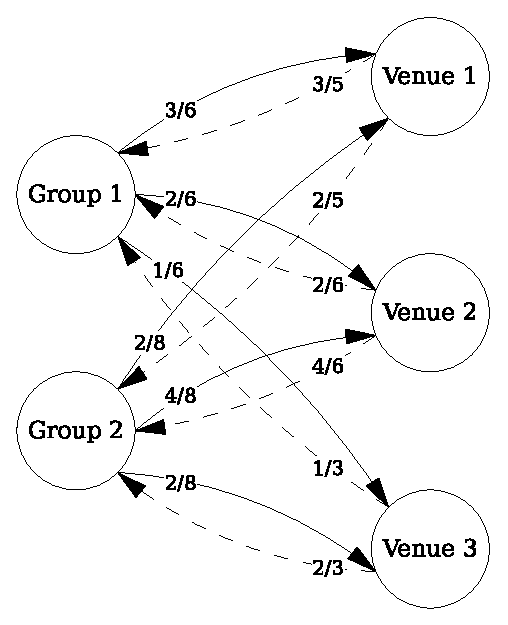
\includegraphics[width=5.5cm]{figures/models/bhrscore-w3}}
   \centerline{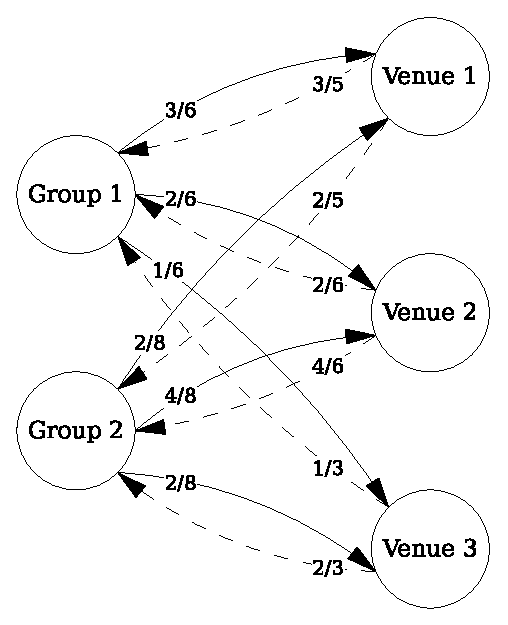
\includegraphics[width=5.2cm]{figures/models/bhrscore-w3}}
   \caption{Markov chain for an example with 2 research groups and 3 publication venues.}
   \label{fig:ex1-MC}
\end{figure}
%
%From Figure \ref{fig:ex1-MC}, 
Group 1 published $3$ papers in venue $\mbox{v}_1$, $2$ papers in venue $\mbox{v}_2$, and $1$ paper in venue $\mbox{v}_3$. The number of publications of Group 1 is $6$. Venue $\mbox{v}_1$ receives $3$ papers of Group 1, and 2 papers of Group 2. The fractions of publications from groups to venues and from venues to groups are the edge weights. We have:
\[
P =
\left[
\begin{array}{c c | c c c }
0            &0             & \  3/6 & \ 2/6     & \  1/6    \\
0            &0             & \  2/8 & \ 4/8     & \  2/8    \\
\hline
3/5        & \ {2/5\ }       &0         &0           &0       \\
2/6        & \ {4/6\ }       &0         &0           &0       \\
1/3        & \ {2/3\ }       &0         &0           &0       \\
\end{array}
\right]
\]

This stochastic matrix corresponds to the Markov chain displayed in Figure~\ref{fig:ex1-MC}, which can be immediately aggregated to a two-state Markov chain, yielding:
%
\[
P^\prime = 
\left[
\begin{array}{c c }
0.467   & \ 0.533 \\
0.400   & \ 0.600
\end{array}
\right]
\]
\noindent which is the stochastic matrix we use in the solution of Equation (\ref{eq:top-rank}). Recall that the dimension of $P^\prime$ is $T \times T$ and, as such, much smaller than that of $P$ for real size problems. Solving Equation (\ref{eq:top-rank}) and applying Equation~\eqref{eq:venue-rank}, we obtain the ranking for the three venues: 
\begin{equation}
\bgamma\bkt{T} = \langle 0.36, 0.43, 0.21 \rangle
\end{equation}

Venue $\mbox{v}_2$ has the highest rank, followed by $\mbox{v}_1$, and then by $\mbox{v}_3$. We remark that the individual values give the {\em relative reputation} of each publication venue. 
%
When we are insterested in computing the P-scores of collateral nodes in the reputation graph, we use the Equation (\ref{eq:pscore}).


\subsection{Reputation Sources}
\label{sec:rep-sources}

The choice of reputation sources is an important part of the method since 
its composition has a direct impact on the final rankings. 
There is no definitive way to make this choice, because it depends on what we want 
to measure. If we select a group of researchers that is generally considered 
to be prestigious, then we will be transferring this group's prestige across nodes in the 
reputation graph by following their publication patterns. If we select a group of 
researchers that share an interest in a research topic, then we will be privileging
conferences related to this topic in the final ranking. A possible interpretation 
of P-scores in the context of conference ranking is the amount of attention devoted 
to a conference by a reference group of researchers.

To provide a general ranking of CS conferences, we can use top CS departments as 
a reference group.
One way to determine the top CS departments is through a simple randomization procedure.
This procedure starts with all 126 research groups evaluated by the NRC\footnote{http://www.nap.edu/rdp}
in its 2011 evaluation of CS graduate programs in the USA. 
First, we need to instantiate the model described previously with a single difference, 
a subset of 10 groups from the NRC evaluation is chosen randomly and used as reputation sources, while the remaining 116 groups
are used as reputation collaterals. This time we also need to execute the propagation of reputations 
from targets to collaterals with a transition matrix $P\bkt{TC}$ of size $|T|\times |C|$ that represents
relations from venues to the collateral research groups. This matrix can be built the same way
the $P\bkt{ST}$ (sources to targets) matrix is built, that is, by associating authors to research 
groups and their papers to publication venues and taking the relative number of papers published
in each venue as a transition probability.

Observe that the randomization procedure is only needed to
select the source nodes for the calculation of venue P-scores, it has no direct relation with the venue ranking
model described in the last section. A run of that procedure works as follows: 
\begin{enumerate}
\item Randomly select 10 departments from the set of top CS departments and use them as the set $s$ of reputation sources
\item Compute steady state probabilities for all nodes using the method described in the last section
\item Using the steady state probabilities of reputation collaterals as a score, select the 10 nodes with 
highest scores and use them as a new set $s_{new}$ of reputation sources
\item If $s_{new} \not \equiv s$ then $s \leftarrow s_{new}$ and go back to step 1
\item $s_{auto} \leftarrow s_{new}$ 
\item Take $s_{auto}$ as the set of automatically selected reputation sources
\item Exit
\end{enumerate}

We repeated this procedure until the set of top 10 groups no longer changed.
By applying this randomization procedure 100 times to a set of 126 USA graduate programs, 
we ended up with a subset of 12 CS programs that appeared 
among the top 10 at least once, after the process stabilized. These 12 CS programs are
described in Table \ref{tab:departments}.

\begin{table}[ht!]
 \centering
 \begin{tabular}{l l} 
 \toprule
 \# & Department \\ 
 \midrule
 1  & Carnegie Mellon University \\
 2  & Georgia Institute of Technology \\
 3  & Massachusetts Institute of Technology \\
 4  & Stanford University \\
 5  & University of California-Berkeley \\
 6  & University of California-Los Angeles \\
 7  & University of California-San Diego \\
 8  & University of Illinois at Urbana-Champaign \\
 9  & University of Maryland College Park \\
 10 & University of Southern California \\
 11 & University of Michigan-Ann Arbor \\
 12 & Cornell University \\
 \bottomrule
 \end{tabular}
 \caption{Reputation sources obtained with the randomization procedure.}
 \label{tab:departments}
\end{table}

All 12 departments listed above are among the top 5th percentile in the ranking produced by NRC. 
Moreover, the first 8 listed groups appeared among the top 10 at every single run.
This suggests that our recursive procedure is able to take advantage of patterns in the publication 
streams of the various CS departments to determine the most reputable ones in fully automatic fashion.
We further observe that this was done while setting the parameter $d\bkt{T} = 0$. That is, we did 
not use information on citation counts in the model. 

\subsection{Summary} 

The basic idea of the P-score index is to capture the transference of reputation among source, 
target, and collateral nodes through their relationships in academia. In particular, in the 
instantiation used in this work, P-score only takes into account researchers and 
their publication records (i.e., papers in publication venues): given a pre-selected 
set of reference research groups (reputation sources), 
P-score associates weights to venues according to the publications of these research groups, 
producing a ranking of publication venues (reputation targets). Furthermore, these weights could 
also be used to rank other research groups or authors (reputation collaterals).

The reputation of a research group is strongly influenced by the reputation of its members, 
which is largely dependent on their publication records. We assume that:
\begin{enumerate}
\item A research group conveys reputation to a publication venue proportionally to its own reputation.
\item A publication venue conveys reputation to a research group proportionally to its own reputation.
\end{enumerate}

Once a reference group is selected, the reputation of its members is transferred to the venues. 
Recursively, since the reputation of research groups is correlated with the reputation of the 
venues in which they published, the venues transfer reputation to the groups. A score for venues 
can then be computed by solving a system of linear equations relating publication venues and 
research groups in the reputation graph, as exemplified in Section~\ref{sec:example}.


\section{Correlation Between P-score and Citation Based Indices} 
\label{sec:correlation}

Bibliometric indicators can be roughly divided into two types. Popularity indicators 
estimate the diffusion of a venues' articles by measuring the number of
endorsements received by that venue (usually in the form of citation counts). Reputation
indicators are similar, but they also try account for the relative reputations of each
endorsing agent, although the concept of reputation may be hard to define.
We argue in this paper that both perspectives have a complementary nature,
since indicators of different types are measuring similar but distinct aspects of
a venue's scientific relevance. 

We performed a combined analysis of conference rankings in Computer Science based on 
P-score, a reputation indicator, and the H-index, a popularity indicator, 
taking into consideration that the concepts of reputation and popularity are
partially related, but also considering that our interest lies exactly in the points
where they diverge more dramatically. Additionally, 
we provide comparisons between P-score, Total Citations and the Impact Factor
to shed light on the relation between P-score and citation based indices.
In computer-related fields, conferences are important channels of dissemination for cutting-edge
research findings~\cite{Lee2019}. Therefore, conference rankings can be valuable to help
identifying promising research topics and good funding opportunities. 
We chose the H-index as the principal indicator of popularity because of its acceptance 
and availability for conferences in bibliometric search engines such as Google Scholar, 
Web of Science and Scopus. 

The H-index~\cite{Hirsch2005} is a composite index of lifelong scientific contribution that takes 
into account the productivity of researchers and the citation impact of their publications.
A researcher has an H-index value of $ h $ if she has $ h $ publications that have been cited at 
least $ h $ times. For example, if a researcher has published 20 papers that received at least 20 
citations each, then her H-index is 20, assuming that 20 is the highest number for which the 
definition of the H-index holds. A journal's H-index can be computed 
in the same way by considering all publications and their collective citation data over a 
definite period as suggested by Braun et al.~\cite{Braun2006}.
Since the H-index was proposed in 2005, the original paper~\cite{Hirsch2005} was 
cited 7,949 times, which attests to its popularity.\footnote{According to Google Scholar, up to the end of 2017.}

As any scientific impact index, the H-index has advantages and disadvantages. 
Some of its advantages are:

\begin{itemize}
\item The simplicity and intuitiveness of its formulation.
\item The longer citation time window when compared to impact factors.
\item H-index has a good predictive power regarding scientific achievement~\cite{Bornmann2005,Hirsch2007}.
\item Its availability in conference rankings.
\end{itemize}

H-index depends on citations to be calculated, thus it suffers from the 
same problems as any other citation-based indices. Some of its major disadvantages are:

\begin{itemize}
\item H-index does not distinguish citations from prestigious and peripheral journals, thus 
it measures popularity rather than quality, although the concepts can have a significant overlap.
\item The time to first citation can be very long.
\item It is not easy to collect all the relevant information.
\item H-index is field-dependent~\cite{Wendl2007}.
\item Major sources do not always agree on its value~\cite{Bar-Ilan2008}. 
\end{itemize}

We propose to use P-score as a complementary index to deal with some of the problems
presented by citation-based indices such as the H-index.
P-score is an index of reputation among peers based on the publication pattern of a set of
reference groups of researchers, the reputation sources. It differs from other network-based 
indices because the venues' reputations derive exclusively from the reputation sources, which 
allows better control of the actual reputation flows. Additionally, to calculate P-scores we 
do not need any citation data, what makes P-scores easier to obtain than H-indices and avoids 
the problem of lack of data that arises from the long time to first citation.

%%%%
The empirical validation of P-score as a measure of reputation was discussed in the 
article by Ribas et al.~\cite{Ribas2015}.
The effectiveness of P-score as a method of venue ranking was attested by comparing its
performance to the H-index baseline in terms of their normalized discounted cumulative 
gains (nDCG)~\cite{Jarvelin2002} at various ranking cutoffs using ground truth 
data obtained from the Qualis system maintained by CAPES\footnore{http://www.capes.gov.br/}, 
a foundation within the Brazilian Ministry of Education. Qualis is an official
brazilian system that annually classifies publication venues in eight grades. % (A1, A2, B1, B2, B3, B4, B5, C)
The grades are assigned by a committee of experts in each field of knowledge 
following a set of criteria, such as: the number of issues, the number of publications, 
the number of repositories that list this venue, citation information, among others.
Using the reference group of departments listed in Table~\ref{tab:departments} and
no citation information, P-score scored consistently higher than the H-index in every 
ranking cutoff, showing that the rankings produced with P-score more closely
conforms to the proxy reputation measure provided by the Qualis classification system.
Naturally, to understand this evidence as a proof of P-score's ability to capture a
venue's reputation, we must first accept that the Qualis ranking provides a reliable 
measure of venue reputations. The Qualis rankings are carefully produced by a
comittee of specialists, but a different choice of comittee could possibly produce
a slightly different ranking. 

While most researchers can probably agree on the relative reputations of some top conferences 
in their fields of expertise, the distinction gets blurred as we move to lower positions in the
ranking. In fact, any ground truth that tries to capture venue reputations can be questioned 
to some extent on the basis of the subjective nature of the concept of reputation. 
P-score does not impose a particular view on reputation, but it relies on two assumptions: 
1) a research group conveys reputation to a publication venue proportionally
to its own reputation; 2) a publication venue conveys reputation to a research group proportionally 
to its own reputation. Considering that these assumptions are valid, the framework of reputation flows 
assigns reputations to venues based on the publication patterns of the reputation sources. 
% Given that these assumptions are true, it follows from the 
% model definition that venues will be ranked according to the reputations of the reference group. 
In the context of this work, all P-score rankings were produced using a reference group 
of CS departments that are generally considered to be reputable, so these rankings capture
the reputations of Computer Science conferences according to the publication patterns of these 
groups.
% The focus of the present work is to show that different indices can capture different aspects
% of the scientific relevance of a venue (which we call popularity and reputation) and, by
% comparing these indices, which are similar but not identical, we can highlight interesting
% cases where measures based on citation counts may be insufficient to provide a good measure
% of research quality.
%%%%

We conducted experiments to investigate the relationship between P-scores, H-indices, Total Citations
and Impact Factors in conference rankings. In particular, we wanted to estimate the degree of correlation 
between P-scores and citation based indices. The data set consists of 794
Computer Science\footnote{
While our data set is entirely composed of Computer Science conferences, nothing in our method is
particular to this field. That is, our index is applicable to any field of knowledge.
} 
conferences
for which the H-index was available on Google Scholar\footnote{http://scholar.google.com.br}
in 2012. P-scores were calculated with
data obtained from DBLP.\footnote{http://dblp.uni-trier.de} The number of publications,
total number of citations and the Impact Factors were obtained from the Microsoft
Academic Graph.\footnote{http://academic.microsoft.com}
The reputation sources
were selected with the randomization procedure described in the previous section, 
yielding the 12 departments listed in Table \ref{tab:departments}. The Impact Factors 
were calculated over a five year period and they correspond to the yearly 
average number of citations received by articles published in each conference during 
this period.


\subsection{P-score and H-index Behavior}

\begin{figure}[ht]
\centering
  \begin{subfigure}{.475\linewidth}
  \centering
 
    \begin{tikzpicture} [scale=0.6]
      \begin{axis}[
          grid=major, % Display a grid
          grid style={dashed,gray!30}, % Set the style
          xlabel=Theoretical Z-Scores,
          ylabel=Sample Z-Scores,
          label style={font=\large},
          ymin=-3,
          ymax=10
        ]
        \addplot[blue, only marks, mark size=0.75pt] 
        table[x=zscore,y=hindex,col sep=comma] {data/normality.csv}; 

        \draw[dotted]
            (axis cs:\pgfkeysvalueof{/pgfplots/xmin},\pgfkeysvalueof{/pgfplots/xmin}) -- 
            (axis cs:\pgfkeysvalueof{/pgfplots/xmax},\pgfkeysvalueof{/pgfplots/xmax});
      \end{axis}
    \end{tikzpicture}
    \caption{H-index Normal Probability Plot}
    \label{fig:hindex_normality}
  \end{subfigure}
  ~
  \begin{subfigure}{.475\linewidth}
    \begin{tikzpicture} [scale=0.6]
      \begin{axis}[
          grid=major, % Display a grid
          grid style={dashed,gray!30}, % Set the style
          xlabel=Theoretical Z-Scores,
          ylabel=Sample Z-Scores,
          label style={font=\large},
          ymin=-3,
          ymax=10
        ]
        \addplot[blue, only marks, mark size=0.75pt] 
        table[x=zscore,y=pscore,col sep=comma] {data/normality.csv}; 

        \draw[dotted]
            (axis cs:\pgfkeysvalueof{/pgfplots/xmin},\pgfkeysvalueof{/pgfplots/xmin}) -- 
            (axis cs:\pgfkeysvalueof{/pgfplots/xmax},\pgfkeysvalueof{/pgfplots/xmax});
      \end{axis}
    \end{tikzpicture}
    % \caption{P-score}
    \caption{P-score Normal Probability Plot}
    \label{fig:pscore_normality}
  \end{subfigure}
  \caption{Normal Probability Plots}
\end{figure}

We plotted normal probability plots for P-scores and H-indices in the CS conference data set 
to identify departures from normality. A normal probability plot shows the theoretical Z-scores
according to the standard normal quantile function on the horizontal axis. For example, at the 90th
percentile (the value below which 90\% of the observations will fall), the normal distribution has a
Z-score of 1.28, meaning that the distribution value at this point is 1.28 standard deviations above 
the median value. On the vertical axis, if we plot the Z-scores according to the quantile function 
described by our sample, we can verify whether it is consistent with a sample from a normal distribution.

\begin{figure}[ht]
\centering
  \begin{subfigure}{.475\linewidth}  
  \centering
    \begin{tikzpicture} [scale=0.6]
      \begin{axis}[
          grid=major, % Display a grid
          grid style={dashed,gray!30}, % Set the style
          xlabel=Log(Num Publications),
          ylabel=Log(H-index),
          xmin=2.0,
          ymin=0.0,
          xmax=5.0,
          ymax=3.0,
        ]
        \draw[red]
            (axis cs:0,0.3137) -- 
            (axis cs:10,4.6167);
        \addplot[blue, only marks, mark size=0.75pt] 
        table[x=publications,y=hindex,col sep=comma] {data/hindex_power_law.csv}; 
        \node[above,red] at (215,50) { $ R^2 = 0.3636 $ };
        \node[above,red] at (230,20) { $ \text{Pearson} = 0.6030 $ };
  
      \end{axis}
    \end{tikzpicture}
    \caption{H-index}
    \label{fig:hindex_powerlaw}
  \end{subfigure}
  ~
  \begin{subfigure}{.475\linewidth}
  \centering
    \begin{tikzpicture} [scale=0.6]
      \begin{axis}[
          grid=major, % Display a grid
          grid style={dashed,gray!30}, % Set the style
          xlabel=Log(Num Publications),
          ylabel=Log(P-score),
          xmin=2.0,
          ymin=0.0,
          xmax=5.0,
          ymax=4.0,
        ]
        \draw[red]
            (axis cs:0,0.2671) -- 
            (axis cs:10,5.7921);
        \addplot[blue, only marks, mark size=0.75pt] 
        table[x=publications,y=pscore,col sep=comma] {data/pscore_power_law.csv}; 
        \node[above,red] at (215,60) { $ R^2 = 0.2705 $ };
        \node[above,red] at (230,20) { $ \text{Pearson} = 0.5201 $ };

      \end{axis}
    \end{tikzpicture}
    \caption{P-score}
    \label{fig:pscore_powerlaw}
  \end{subfigure}
  \caption{
    Log(H-index) versus Log(Num Publications) for the CS conferences only considering conferences with more 
    than 1000 publications and averaging the number of publications for conferences with identical indices.}
  \label{fig:powerlaw}
\end{figure}

We compared theoretical and sample Z-scores for 794 quantiles (one for each data point) in Figures
\ref{fig:hindex_normality} and \ref{fig:pscore_normality}. The dotted line is the identity line for
which sample and theoretical Z-scores converge. As becomes clear from the plots, both distributions
are significantly skewed, indicating that P-scores and H-indices do not follow normal distributions.
In fact, the values of H-indices and P-scores tend to increase with the number of publications $ N $ 
and their behavior is better described by a power-law model: 
%
\begin{equation}
X_i = C \times N_i^a
\end{equation}
%
where $ C $ and $ a $ are index-specific constants, $ X_i $ is the index value and $ N_i $ is the 
number of publications for observation $ i $. Figure~\ref{fig:powerlaw} presents the 
log-log plots for P-scores and H-indices versus the number of publications. A linear 
relationship between the logarithms indicate a power-law behavior. The estimated parameters
for the constants of the power-law model in the best linear fit are 
$ C = 2.0591 $ and $ a = 0.4303 $ for the H-index,
$ C = 1.8498 $ and $ a = 0.5525 $ for P-score.

The tendence of P-scores and H-indices to increase with the number of publications may hurt the comparison of venues 
with a largely different size, obfuscating less prolific conferences. To account for this fact, we also plot 
correlations for the normalized P-scores and H-indices using a measure called the Scientific Performance 
QuaLity (SPQL) level~\cite{Babic2016}.
Originally, the SPQL level only handles H-indices, but we also use it as a normalization procedure for
P-score. The SPQL level can be defined as:
%
\begin{equation}
SPQL(i) = 100 \cdot \frac{\tilde{X_i}}{X_i}
\end{equation}
%
where $ \tilde{X_i} $ is the observed value for the index in point $ i $ and $ X_i $ is the corresponding
value in the best fit line. In our case, 
$ X_i = 2.0591 \times N_i^{0.4303} $ for the H-index and 
$ X_i = 1.8498 \times N_i^{0.5525} $ for P-score.
This way, we have a measure that indicates
the degree of deviation from average that is independent of the number of publications and allows
the comparison of venues with different sizes.


\subsection{P-score Correlations}

\begin{figure}[!ht]
\centering
  \begin{subfigure}{.475\linewidth}  
  \centering
    \begin{tikzpicture} [scale=0.6]
      \begin{axis}[
          grid=major, % Display a grid
          grid style={dashed,gray!30}, % Set the style
          xlabel=H-index Ranks,
          ylabel=Total Citations Ranks,
          xmin=-100,
          ymin=-100,
          xmax=900,
          ymax=900
        ]
        \addplot[blue, only marks, mark size=0.75pt] 
        table[x=hindex,y=citations,col sep=comma] {data/ranks.csv}; 

      \end{axis}
    \end{tikzpicture}
    \caption{H-index $ \times $ Total Citations}
  \end{subfigure}
  ~
  \begin{subfigure}{.475\linewidth}  
  \centering
    \begin{tikzpicture} [scale=0.6]
      \begin{axis}[
          grid=major, % Display a grid
          grid style={dashed,gray!30}, % Set the style
          xlabel=H-index Ranks,
          ylabel=Impact Factor Ranks,
          xmin=-100,
          ymin=-100,
          xmax=900,
          ymax=900
        ]
        \addplot[blue, only marks, mark size=0.75pt] 
        table[x=hindex,y=perpaper,col sep=comma] {data/ranks.csv}; 

      \end{axis}
    \end{tikzpicture}
    \caption{H-index $ \times $ Impact Factor}
  \end{subfigure}

  \vspace{0.4cm}%

  \begin{subfigure}{.475\linewidth}  
  \centering
    \begin{tikzpicture} [scale=0.6]
      \begin{axis}[
          grid=major, % Display a grid
          grid style={dashed,gray!30}, % Set the style
          xlabel=P-score Ranks,
          ylabel=Total Citation Ranks,
          xmin=-100,
          ymin=-100,
          xmax=900,
          ymax=900,
        ]
        \addplot[blue, only marks, mark size=0.75pt] 
        table[x=pscore,y=citations,col sep=comma] {data/ranks.csv}; 

      \end{axis}
    \end{tikzpicture}
    \caption{P-score $ \times $ Total Citations}
  \end{subfigure}
  ~
  \begin{subfigure}{.475\linewidth}  
  \centering
    \begin{tikzpicture} [scale=0.6]
      \begin{axis}[
          grid=major, % Display a grid
          grid style={dashed,gray!30}, % Set the style
          xlabel=P-score Ranks,
          ylabel=Impact Factor Ranks,
          xmin=-100,
          ymin=-100,
          xmax=900,
          ymax=900,
        ]
        \addplot[blue, only marks, mark size=0.75pt] 
        table[x=pscore,y=perpaper,col sep=comma] {data/ranks.csv}; 

      \end{axis}
    \end{tikzpicture}
    \caption{P-score $ \times $ Impact Factor}
  \end{subfigure}

  \vspace{0.4cm}%

  \begin{subfigure}{.475\linewidth}
  \centering
    \begin{tikzpicture} [scale=0.6]
      \begin{axis}[
          grid=major, % Display a grid
          grid style={dashed,gray!30}, % Set the style
          xlabel=P-score Ranks,
          ylabel=H-index Ranks,
          xmin=-100,
          ymin=-100,
          xmax=900,
          ymax=900,
        ]
        \addplot[blue, only marks, mark size=0.75pt] 
        table[x=pscore,y=hindex,col sep=comma] {data/ranks.csv}; 

      \end{axis}
    \end{tikzpicture}
    \caption{P-score $ \times $ H-index}
  \end{subfigure}
  ~
  \begin{subfigure}{.475\linewidth}
  \centering
    \begin{tikzpicture} [scale=0.6]
      \begin{axis}[
          grid=major, % Display a grid
          grid style={dashed,gray!30}, % Set the style
          xlabel=SPQL P-score Ranks,
          ylabel=SPQL H-index Ranks,
          xmin=-100,
          ymin=-100,
          xmax=900,
          ymax=900,
        ]
        \addplot[blue, only marks, mark size=0.75pt] 
        table[x=pscore,y=hindex,col sep=comma] {data/normalized.csv}; 

      \end{axis}
    \end{tikzpicture}
    \caption{SPQL P-score $ \times $ SPQL H-index}
  \end{subfigure}
  \caption{
  Scatter plots comparing the rankings produced with P-scores, H-indices, Total Citations 
  and Impact Factors in a set of 794 conferences in Computer Science.
  }
  \label{fig:scatter_plots}
\end{figure}

We studied the correlation between P-score and various citation-based indices 
in the context of Computer Science conference ranking to understand how reputation
and popularity indices diverge, and to understand if the combined assessment of 
reputation and popularity indices can reveal interesting conferences that are
not perceived in the rankings produced with a single index.

\begin{table}[ht!]
  \small
  \centering
  \begin{tabular}{lllll} 
  \toprule
  First & Second & Kendall-Tau & Spearman & Pearson \\ 
  \midrule
  H-index     & Total Citations           & 0.6141 & 0.7623 & 0.6848 \\
  H-index     & Impact Factor             & 0.3786 & 0.5306 & 0.5276 \\ 		
  P-score     & Total Citations           & 0.5028 & 0.6751 & 0.7798 \\
  P-score     & Impact Factor             & 0.3353 & 0.4851 & 0.3120 \\ 		
  P-score     & H-index                   & 0.5153 & 0.6939 & 0.7089 \\
  SPQL Pscore & SPQL H-index              & 0.4148 & 0.5822 & 0.4957 \\
  \bottomrule
  \end{tabular}
  \caption{Correlations between P-scores, H-index, Total Citations 
  and Impact Factors in a set of 794 conferences in Computer Science.}
  \label{tab:correlations}
\end{table}

Figure~\ref{fig:scatter_plots} compares rankings of the 794 CS conferences in terms of their
P-score, H-index, Total Citations and Impact Factors.
Points that are closer to the origin have better ranks (i.e. a data point at position 1 is 
better ranked than a data point at position 200). Also, Table~\ref{tab:correlations} presents the
correlations between indices in terms of their Kendall-Tau, Spearman and Pearson coefficients.
The Spearman coefficient is essentially a Pearson Correlation of ranking positions. The
Kendall-Tau is another correlation measure based on ranks that is deemed less
sensitive to errors than the Spearman coefficient~\cite{Kendall1955,Baeza-Yates2011}. These 
correlation coefficients assume a value between -1 and 1. A value of 1 indicates that two rankings are 
identical and a value of -1 indicates that rankings are the inverse of each other, with values 
inbetween indicating partial correlation. A coefficient close to zero indicates no correlation.

The first fact to point out is that H-indices are significantly correlated to the Total Citations
received by a conference but not as much to the Impact Factor,
what is also observed in P-score. Both indices seem to be somewhat reliant on the number of 
publications, so it is not unexpected that they are less correlated to Impact Factors
than to Total Citation counts. 

Also, P-scores seem to be quite correlated to H-indices, assuming a Kendall-Tau of 0.5153.
The Kendall-Tau is defined in terms of concordant and discordant pairs of ranks.
P-scores agree aproximately 76\% of the time with H-indices on which conference should be
ranked above the other. However, normalized P-scores and H-indices in the form of the SPQL
measure have a significantly smaller degree of correlation (a Kendall-Tau of 0.4148) 
showing that, once we control for the number of publications, P-scores and H-indices seem
to be more clearly capturing different aspects of a conference's scientific impact. 

In our assessment, we are especially interested in conferences for which popularity 
and reputation measures are most disagreeing. These would be conferences with high P-scores 
and low H-indices or high H-indices and low P-scores. These interesting outliers can both
be captured by plotting H-indices against P-scores or the normalized version of the measures.
We will proceed in the next Section with the assessment of P-scores versus H-indices.


\section{Assessing Conferences in CS}
\label{sec:notifications}


\begin{figure}[ht]
\centering
  \begin{subfigure}{.475\linewidth}
  \centering
    \begin{tikzpicture} [scale=0.6]
      \begin{axis}[
          grid=major, % Display a grid
          grid style={dashed,gray!30}, % Set the style
          xlabel=P-score ranks,
          ylabel=H-index ranks
          xmin=-100,
          ymin=-100,
          xmax=900,
          ymax=900,
        ]
        \draw[red]
            (axis cs:0,0) -- 
            (axis cs:1732.0508,1000);
        \draw[red]
            (axis cs:0,0) -- 
            (axis cs:1000,1732.0508);
        \addplot[blue, only marks, mark size=0.75pt] 
        table[x=pscore,y=hindex,col sep=comma] {data/ranks.csv}; 

      \end{axis}
    \end{tikzpicture}
    \caption{Angle strategy for delimiting our three groups of interest: Top, Center and Bottom - with pivot at the origin.}
    \label{fig:angle_strategy}
  \end{subfigure}
  ~
  \begin{subfigure}{.475\linewidth}  
  \centering
    \begin{tikzpicture} [scale=0.6]
      \begin{axis}[
          grid=major, % Display a grid
          grid style={dashed,gray!30}, % Set the style
          xlabel=P-score ranks,
          ylabel=H-index ranks
          xmin=-100,
          ymin=-100,
          xmax=900,
          ymax=900,
        ]
        \draw[red]
            (axis cs:-100,-100) -- 
            (axis cs:1632.05081,900);
        \draw[red]
            (axis cs:-100,-100) -- 
            (axis cs:900,1632.0508);
        \addplot[blue, only marks, mark size=0.75pt] 
        table[x=pscore,y=hindex,col sep=comma] {data/ranks.csv}; 
  
      \end{axis}
    \end{tikzpicture}
    \caption{Angle strategy for delimiting our three groups of interest with pivot positioned behind the origin, at point (-100, -100).}
    \label{fig:angle_strategy_adapted}
  \end{subfigure}
\end{figure}

\begin{figure}[ht!]
  \begin{center}
    \begin{tikzpicture} 
      \begin{axis}[
          grid=major, % Display a grid
          grid style={dashed,gray!30}, % Set the style
          xlabel=P-score ranks,
          ylabel=H-index ranks,
          xmin=-100,
          ymin=-100,
          xmax=900,
          ymax=900,
          width=12cm,height=12cm
        ]
        \addplot[
          blue, only marks, mark size=0.75pt
        ] 
        table[x=pscore,y=hindex,col sep=comma] {data/ranks.csv}; 
        \addplot[
          red, only marks, mark size=0.75pt,
          nodes near coords*={\Label},
          visualization depends on={value \thisrow{label} \as \Label},
          style={font=\tiny}
        ] 
        table[x=pscore,y=hindex,col sep=comma] {data/ranks.csv}; 

      \end{axis}
    \end{tikzpicture}
    \caption{P-score ranks $ \times $H-index ranks scatter plot with markings showing conference names.}
    \label{fig:markings}
  \end{center}
\end{figure}

Since P-scores and H-indices are fairly correlated, most data points in our example are clustered close to the identity 
line, showing an apparent agreement between the indices. However, there are noticeable differences, 
particularly in those cases for which the P-score rank position is high and the H-index rank is low,
or for which the H-index rank is high and the 
P-score rank is low. Therefore, we 
can distinguish between three groups of interest in the data set:
%
\begin{itemize}
\item \textit{Center Group}: highly correlated data points. These are the 
venues that are popular (i.e. high H-index) and reputable (i.e. high P-score), 
or venues that are unpopular and not very reputable.
\item \textit{Top Group}: venues with a high P-score and low H-index. These 
are the venues that are reputable (i.e. endorsed by researchers at top CS departments), 
but not very popular.
\item \textit{Bottom Group}: venues with a high H-index and low P-score. 
These are the venues that are popular, but not very reputable in the sense 
that they are not endorsed by the reputation sources.
\end{itemize}
%

\subsection{Delimitation of Interest Groups}
\label{ssec:delimitation_strategy}

We devised a strategy for delimiting the Top, Center and Bottom sets. 
It consists of drawing two line segments, starting from
the origin, separated by an angle $ \theta $, and examining
how the correlation between the data points in the 
Center Group varies with respect to variations in the angle 
$ \theta $. It is what we call the "angle strategy", as 
illustrated in Figure \ref{fig:angle_strategy}. We immediately 
notice several data points close to the origin
which are not included in the Center Group. This is a problem, 
given that these points correspond to CS conferences that have a high H-index rank and a high
P-score rank and thus, are strongly correlated. To
correct this, we move the point where the lines meet, which we also
refer to as the pivot, to a point behind the origin, one
such as (-100, -100), as illustrated in Figure \ref{fig:angle_strategy_adapted}. 
By doing so, we ensure that all data points near the origin are included in the
Center Group.

\begin{table}[ht!]
\centering
 \begin{tabular}{c c c c} 
 \toprule
 Angle & Kendall-Tau & Spearman & Items in center group \\ 
 \midrule
 90 & 0.5153 & 0.6939 & 794 \\ 
 80 & 0.5153 & 0.6939 & 794 \\
 70 & 0.5186 & 0.6989 & 793 \\
 60 & 0.5269 & 0.7094 & 790 \\
 50 & 0.5523 & 0.7341 & 777 \\
 40 & 0.5884 & 0.7611 & 749 \\
 30 & 0.6510 & 0.7998 & 689 \\
 20 & 0.7290 & 0.8295 & 576 \\
 10 & 0.8434 & 0.8481 & 345 \\
 \bottomrule
 \end{tabular}
 \caption{Angle strategy Kendall-Tau in center group by varying the angle.}
 \label{tab:angle_strategy}
\end{table}

Table \ref{tab:angle_strategy} describes how the Kendall-Tau and Spearman coefficients vary for items 
in the Center Group, as we vary the angle $ \theta $, with the pivot positioned behind 
the origin as in Figure \ref{fig:angle_strategy_adapted}. We notice that for $ \theta = 30^{\circ} $, 
689 conferences are included in the Center
Group (close to 87\% of all conferences in the data set). What leaves only a handful of conferences to
be analyzed individually outside the Center Group.
Thus, in our subsequent 
analysis, we employed the angle strategy with $ \theta = 30^{\circ} $, since it provides 
a good trade off between correlation and coverage in our data set.

\begin{table}[ht!]
  \small
  \centering
  \begin{tabular}{c c c c} 
  \toprule
  \# & Top & Center & Bottom \\ 
  \midrule
  1  & IROS      & ICRA        & IPTPS   \\
  2  & ICMCS     & CHI         & MOBIHOC \\
  3  & ISIT      & CVPR        & ACSAC   \\
  4  & ICCD      & AAAI        & ICWS    \\
  5  & CDC       & NIPS        & ISM     \\
  6  & ICPP      & DAC         & ISMIR   \\
  7  & WCNC      & ICASSP      & PIMRC   \\
  8  & LCPC      & STOC        & BIBE    \\
  9  & ISQED     & FOCS        & DFT     \\
  10 & ISER      & INTERSPEECH & FSKD    \\
  11 & WACV      & ICCAD       & ICIDS   \\
  12 & ITS       & IJCAI       & MMM     \\
  13 & ICWSM     & SODA        & ECIS    \\
  14 & AIED      & INFOCOM     & ISVLSI  \\
  15 & GIS       & ICML        & IHI     \\
  16 & CCCG      & ICIP        & MMVR    \\
  17 & DCC       & SIGMOD      & ARC     \\
  18 & HUMANOIDS & ICSE        & VNC     \\
  19 & LREC      & IPPS        & IAT     \\
  20 & WAFR      & ICCV        & ICAI    \\
  21 & WSDM      & ICDE        & ICA3PP  \\
  22 & CICC      & ACL         & ANALCO  \\
  23 & MMSP      & ECCV        & CNSR    \\
  24 & CLUSTER   & ISCA        & ICEBE   \\
  25 & CONLL     & KDD         & PAAP    \\
  26 & CLOUD     & SIGCOMM     & PROMAS  \\
  27 & MFCS      & SC          & WI      \\
  28 & FSR       & WWW         & WKDD    \\
  29 & ICAC      & ICDCS       & APSCC   \\
  30 & WABI      & DATE        & CATA    \\
  \bottomrule
  \end{tabular}
  \caption{Conferences (short names) ranked by P-score in the bottom, center and top groups.}
  \label{tab:conferences}
\end{table}

With the pivot positioned at (-100, -100) and $ \theta=30^{\circ} $, the Top Group ended with 56 conferences, the 
Center Group with 689 conferences, and the Bottom Group with 49 conferences. Table 
\ref{tab:conferences} presents the top 30 conferences, ranked by P-score, for each of the three groups
and Figure~\ref{fig:markings} shows the P-score $ \times $ H-index scatter plots showing all conference
names for the Bottom and Top groups.

The Center Group consists of conferences that have a high correlation between reputation and
popularity. The reputation of these conferences is well represented by the number of citations
they receive. This group represents conferences that are relatively easy to classify regarding
their scientific impact. Among them we find WWW, CVPR and KDD, to name a few.

The Top Group consists of conferences with a high P-score rank and low H-index rank. While these conferences
receive a relatively low number of citations, reputable researchers 
(i.e. our reference set of top research groups in Computer Science) still publish 
in them consistently, as we can observe from their high P-score ranks. The primary reason is that
conferences in the Top Group are usually venues associated with smaller subareas of Computer Science, 
and are therefore venues that receive a smaller number of citations. Because of that, their H-indices 
tend to be smaller and their H-index rank positions tend to be worse. Despite that, many of these 
venues might have a high reputation in their subareas and thus, high P-scores. 
For example, ICPP, and LCPC are conferences related to parallel processing that capture
considerable attention from the top CS departments, as we can observe from their high P-scores. 
Similarly IROS, WAFR, and HUMANOIDS are conferences in Robotics that have high P-scores
and relatively low H-indices. These conferences may end up being neglected by funding councils and 
committees in their assessment if we look only at the H-index, because these subareas do not receive 
as many citations as others.

% The total number of publications in Parallel Processing is comparatively low 
% compared to other subareas of Computer Science such as Algorithms or Database 
% Management Systems~\cite{Hoonlor2013}. 
% So, it is reasonable to assume that conferences 
% in this subarea are expected to receive fewer citations than their counterparts in more popular subareas.
% P-scores can assist human evaluators with funding decisions by shedding light on these conferences.

The Bottom Group consists of conferences with a low P-score rank and high H-index rank. These conferences
receive a high number of citations, but their reputation among top computer scientists is comparatively low, 
as reflected by their P-scores. Conferences in this
group are usually situated in the intersection between Computer Science and other areas of knowledge. Some examples of such venues are
BIBE, related to Biocomputing, IHI, MMVR, related to Health, and
DFT, and VNC which are related to Engineering and Electronics. Because these are large research communities, venue H-indices tend to be 
relatively high (particularly with regard to Computer Science). In the case of these events, funding councils in Computer Science should consider not only the high H-indexes, but also the venue reputation among computer
scientists. Indeed, an exceptionally popular and reputable conference in electronics may not be as 
popular or prestigious when being considered from the point of view of computer scientists. That is, P-scores may aid 
human evaluators with funding decisions by pinpointing conferences that intersect multiple areas of knowledge and by providing
an estimate of the conference's reputation among peers in the field of interest.

\subsection{P-score on a Per Subarea Basis}

In the previous experiments, we showed how to use P-score as a complementary 
index to citation-based indicators, such as H-index, to assess the reputation 
of conferences in Computer Science. However, it is important to note that the 
index P-score captures the transference of reputation \textit{from} source nodes 
\textit{to} target and collateral nodes. Therefore, the choice of reputation 
sources defines the context where the reputation flows will be assessed and 
it can be adjusted to specific information needs. In this article, we used P-score 
to investigate Computer Science conference reputations from the point of view of
a general reference set of computer scientists. But,
%it is common that a funding council has to distinguish
one could be interested, for example, in determining which are the most relevant conferences 
in a given \textit{subarea} of Computer Science. This is an important piece of 
information for funding councils when evaluating the productivity of individual 
researchers or research groups. In contrast to H-index, P-score is capable 
of producing results on a per subarea basis. % if starting from highly reputable sources

\begin{table}[ht]
  \small
  \centering
  \begin{tabular}{c c c } 
  \toprule
  Natural Language Processing  & Machine Learning & Information Retrieval  \\ 
  \midrule
  NIPS & NIPS & SIGIR \\
  ACL  & ICML & CIKM \\
  EMNLP & CVPR & WWW \\
  ICML  & ECCV & SIGMOD \\
  NAACL & ICCV & VLDB \\
  INTERSPEECH & ICASSP & ICDE \\
  CONLL  & BMVC & TREC \\
  ICASSP  & IJCAI & WSDM \\
  ICANN  & AAAI & ECIR \\
  IJCNN  & ICANN & KDD \\
  \bottomrule
  \end{tabular}
  \caption{Conferences (short names) selected by P-score in three subareas of Computer Science.}
  \label{tab:subareas}
\end{table}

In Table~\ref{tab:subareas}, we show different sets of conferences in Computer Science highly ranked by P-score in three subareas: Natural Language Processing (NLP), Machine Learning (ML), and Information Retrieval (IR). In this experiment, we used as reputation sources the first ten individual researchers in each subarea according to Microsoft Academic.\footnote{http://academic.microsoft.com/authors} % in terms of \textit{saliency}, a measure of research impact that leverages the [xxx]. 
Indeed, although the information available in Microsoft Academic was used in this experiment, there are other effective strategies to choose the reputation sources, such as: i) to ask experts in each subarea to provide a list of the most reputable researchers and then aggregate the results using a voting method, ii) to use curated lists of impactful researchers in each subarea (when available), iii) to build a list only with awarded researchers in each subarea.

With a few reputation sources, P-score can correctly find reputable conferences on each subarea of knowledge, a problem that has been the subject of study in the literature~\cite{wainer13,leydesdorff13,waltman13}. Moreover, we can find conferences with low popularity but high reputation, such as CONLL in NLP, ICANN in ML, and WSDM in IR. On the other hand, well-known conferences that have both popularity and reputation within their respective subareas are also presented, as expected --- e.g., ACL and INTERSPEECH in NLP, ICML and CVPR in ML, NIPS both in NLP and ML, SIGIR and CIKM in IR. This information may be useful to support decisions of research funding councils focused on specific subareas instead of broad areas of knowledge by assessing the subarea-specific P-scores in comparison with conference H-indices, as presented in Section~\ref{ssec:delimitation_strategy}. It is noteworthy that these subarea-specific rankings were produced with only a small subset of reputable researchers to demonstrate the flexibility of P-scores, however they should not be taken authoritatively.

% It is noteworthy that these subarea-specific ranking should not be considered as standard rankings of conferences for each subarea. Instead, similarly to the results for the broad area of Computer Science, these results should be used to complement other indicators, such as H-index, on a per subarea basis. 

% NN: NIPS ICML  CVPR ICASSP ECCV AAAI ICANN INTERSPEECH UAI ESANN
% \begin{table}[ht!]
%   \small
%   \centering
%   \begin{tabular}{c c c c c} 
%   \toprule
%   \# & NLP & NN & ML & IR  \\ 
%   \midrule
%   1  & ACL & NIPS & NIPS & SIGIR \\
%   2  & NAACL & ISNN & KDD & TREC \\
%   3  & EMNLP & IJCNN & ICDM & CIKM \\
%   4  & LREC & CDC & ICDE & ECIR \\
%   5  & INTERSPEECH & ISCAS & ICML & WWW \\
%   6  & COLING & ICML & SDM & WSDM \\
%   7  & CONLL & ICRA & SIGMOD & RIAO \\
%   8  & ICASSP & ADPRL & CIKM & NAACL \\
%   9  & AAAI & IEEEISIC & VLDB & KDD \\
%   10 & IWSLT & ICANN & UAI & CHI \\
%   \bottomrule
%   \end{tabular}
%   \caption{Conferences (short names) ranked by P-score (top10 authors by MS H-Index) in four CS subareas: NLP, Art. NN, IR, and ML.}
%   \label{tab:subareas-hindex}
% \end{table}
% \begin{table}[ht!]
%   \small
%   \centering
%   \begin{tabular}{c c c c c | c c c c} 
%   \toprule
%   \# & NLP & NN & ML & IR & NLP & NN & ML & IR \\ 
%   \midrule
%   1  & ACL	&	VPR	&	CVPR	&	SIGIR	&	ACL	&	NeurIPS	&	NeurIPS	&	SIGIR\\
%   2  & EMNLP	&	NeurIPS	&	NeurIPS	&	CIKM	&	EMNLP	&	SMC	&	ICML	&	WWW\\
%   3  & NAACL	&	ICLR	&	ICML	&	WWW	&	NAACL	&	IJCNN	&	CVPR	&	CIKM\\
%   4  & LREC	&	IJCNN	&	AAAI	&	TREC	&	COLING	&	CVPR	&	SMC	&	TREC\\
%   5  & COLING	&	ICML	&	SMC	&	VLDB	&	LREC	&	ICASSP	&	KDD	&	VLDB\\
%   6  & INTERSPEECH	&	ICASSP	&	ICLR	&	SIGMOD	&	INTERSPEECH	&	ICLR	&	ECCV	&	SIGMOD\\
%   7  & IJCNLP	&	SMC	&	KDD	&	ACL	&	ICASSP	&	ICML	&	AAAI	&	ACL\\
%   8  & ICLR	&	INTERSPEECH	&	ECCV	&	WSDM	&	EACL	&	ISNN	&	IJCAI	&	MM\\
%   9  & NeurIPS	&	ISNN	&	ACL	&	ECIR	&	AAAI	&	ICRA	&	ACL	&	WSDM\\
%   10 & AAAI	&	ICCV	&	ICCV	&	MM	&	IJCNLP	&	INTERSPEECH	&	ICCV	&	ICDE\\
%   \bottomrule
%   \end{tabular}
%   \caption{(Left) Conferences ranked by MS by Saliency and (right) by H-index.}
%   \label{tab:subareas-hindex}
% \end{table}

\section{Conclusions}
\label{sec:conclusions}

We have compared the P-scores and H-indices of 794 conferences in Computer Science to
understand how P-score, a reputation based index that does not rely on citation data, can be 
used in conjunction with citation based indices to provide insight on scientific impact
assessment.
We found that P-score and H-index have a significant correlation reflected 
by a Kendall-Tau of approximately 0.5153. However,
there are important differences between the two indices.
Our interpretation of these results are based on the intuition that while H-indices 
provide a quantification of the popularity of a publication or researcher among their 
peers, P-scores provide a quantification of the reputation of a publication or 
researcher among peers.
We can distinguish three separate cases. First, when P-scores and 
H-indices agree, we find venues that have proportionate amounts of popularity and 
reputation among computer scientists. Second, when P-scores 
are high (better rank position) and H-indices are low (worse rank position) we have 
venues of good reputation among computer scientists that are associated with small 
research communities or subareas. Third, when P-scores are low (worse rank position) 
and H-indices are high, we have venues of good popularity (usually associated with 
large research communities outside Computer Science) that do not stand with a high
reputation among computer scientists, that is, computer scientists do not publish 
frequently there. These differences indicate a complementary aspect to these indices. P-scores, 
used in conjunction with H-indices, allow us to distinguish the three types of 
venues mentioned above. This provides useful information which can be employed
by research funding councils and committees to better understand the scientific relevance 
of venues and researchers and thus, take more informed funding decisions. 

There are several directions for further research using P-score. 
Given the flexibility of P-score to grasp the relative importance of different fields
and subareas, an interesting topic for future research would be to analyze
the development of research interest over time in different fields and countries.
Also, considering that citation counts for newly published articles take at least a couple 
of years to develop and, since P-scores can be promptly obtained, future work
could study the capacity of P-score to predict the future
scientific impact of research articles, venues and authors. This capacity would be especially 
useful to help identifying promising research in advance.

\bibliographystyle{spmpsci}
\bibliography{pscore_correlation}

% \section*{Appendix: Abbreviations}
% \begin{table}[ht]
%   \small
%   \centering
%   \begin{tabular}{ l l } 
%   \toprule
%   Short name  & Full name \\ 
%   \midrule
%   AAAI & Conference on Artificial Intelligence \\ 
%   ACL & Meeting of the Association for Computational Linguistics  \\ 
%   BMVC & British Machine Vision Conference \\ 
%   CIKM & International Conference on Information and Knowledge Management \\ 
%   CONLL & Computational Natural Language Learning \\ 
%   CVPR & Computer Vision and Pattern Recognition \\ 
%   ECCV & European Conference on Computer Vision \\ 
%   ECIR & European Conference on IR Research \\ 
%   EMNLP & Empirical Methods in Natural Language Processing \\ 
%   ICANN & International Conference on Artificial Neural Networks \\ 
%   ICASSP & International Conference on Acoustics, Speech, and Signal Processing \\ 
%   ICCV & IEEE International Conference on Computer Vision \\ 
%   ICDE & International Conference on Data Engineering \\ 
%   ICML & International Conference on Machine Learning \\ 
%   IJCAI & International Joint Conference on Artificial Intelligence \\ 
%   IJCNN & International Joint Conference on Neural Networks \\ 
%   INTERSPEECH & International Speech Communication Association \\ 
%   KDD & Knowledge Discovery and Data Mining \\ 
%   NAACL & North American Chapter of the Association for Computational Linguistics \\ 
%   NIPS & Neural Information Processing Systems (NeurIPS) \\ 
%   SIGIR & International Conference on Research and Development in Information Retrieval  \\ 
%   SIGMOD &  International Conference on Management of Data \\ 
%   TREC & Text REtrieval Conference \\ 
%   VLDB & Very Large Data Bases Conference  \\ 
%   WSDM & Web Search and Data Mining \\ 
%   WWW & International World Wide Web Conferences \\
%   \bottomrule
%   \end{tabular}
%   % \caption{}
%   \label{tab:subareas-saliency}
% \end{table}


\end{document}
